% Created by tikzDevice version 0.12.3 on 2020-03-29 17:27:31
% !TEX encoding = UTF-8 Unicode
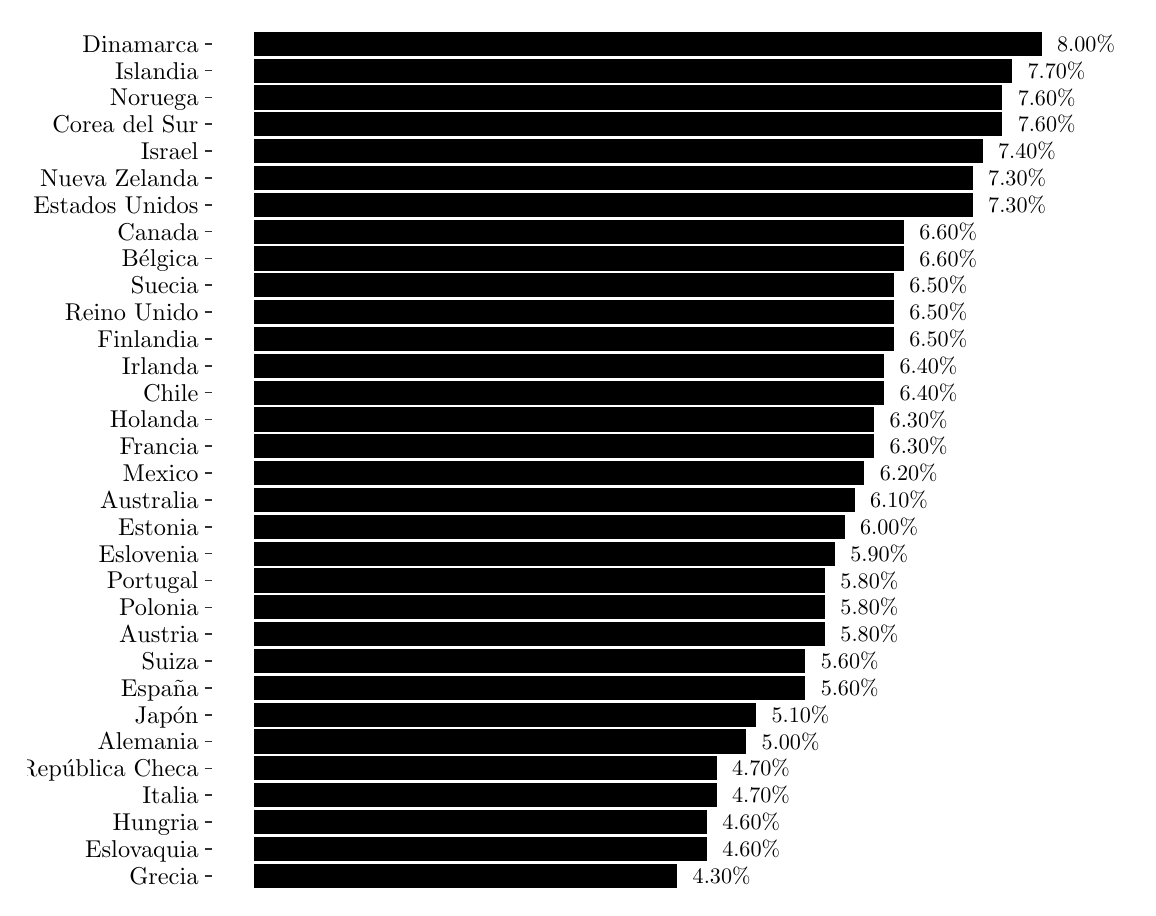
\begin{tikzpicture}[x=1pt,y=1pt]
\definecolor{fillColor}{RGB}{255,255,255}
\path[use as bounding box,fill=fillColor,fill opacity=0.00] (0,0) rectangle (397.48,310.76);
\begin{scope}
\path[clip] (  0.00,  0.00) rectangle (397.48,310.76);
\definecolor{fillColor}{RGB}{255,255,255}

\path[fill=fillColor] ( -0.00,  0.00) rectangle (397.48,310.76);
\end{scope}
\begin{scope}
\path[clip] ( 66.68,  0.00) rectangle (397.48,310.76);
\definecolor{fillColor}{RGB}{255,255,255}

\path[fill=fillColor] ( 66.68, -1.50) rectangle (397.48,310.76);
\definecolor{drawColor}{RGB}{255,255,255}

\path[draw=drawColor,line width= 0.3pt,line join=round] (117.30,  0.00) --
	(117.30,310.76);

\path[draw=drawColor,line width= 0.3pt,line join=round] (188.48,  0.00) --
	(188.48,310.76);

\path[draw=drawColor,line width= 0.3pt,line join=round] (259.66,  0.00) --
	(259.66,310.76);

\path[draw=drawColor,line width= 0.3pt,line join=round] (330.84,  0.00) --
	(330.84,310.76);

\path[draw=drawColor,line width= 0.6pt,line join=round] ( 66.68,  4.31) --
	(397.48,  4.31);

\path[draw=drawColor,line width= 0.6pt,line join=round] ( 66.68, 14.01) --
	(397.48, 14.01);

\path[draw=drawColor,line width= 0.6pt,line join=round] ( 66.68, 23.71) --
	(397.48, 23.71);

\path[draw=drawColor,line width= 0.6pt,line join=round] ( 66.68, 33.41) --
	(397.48, 33.41);

\path[draw=drawColor,line width= 0.6pt,line join=round] ( 66.68, 43.10) --
	(397.48, 43.10);

\path[draw=drawColor,line width= 0.6pt,line join=round] ( 66.68, 52.80) --
	(397.48, 52.80);

\path[draw=drawColor,line width= 0.6pt,line join=round] ( 66.68, 62.50) --
	(397.48, 62.50);

\path[draw=drawColor,line width= 0.6pt,line join=round] ( 66.68, 72.20) --
	(397.48, 72.20);

\path[draw=drawColor,line width= 0.6pt,line join=round] ( 66.68, 81.90) --
	(397.48, 81.90);

\path[draw=drawColor,line width= 0.6pt,line join=round] ( 66.68, 91.59) --
	(397.48, 91.59);

\path[draw=drawColor,line width= 0.6pt,line join=round] ( 66.68,101.29) --
	(397.48,101.29);

\path[draw=drawColor,line width= 0.6pt,line join=round] ( 66.68,110.99) --
	(397.48,110.99);

\path[draw=drawColor,line width= 0.6pt,line join=round] ( 66.68,120.69) --
	(397.48,120.69);

\path[draw=drawColor,line width= 0.6pt,line join=round] ( 66.68,130.38) --
	(397.48,130.38);

\path[draw=drawColor,line width= 0.6pt,line join=round] ( 66.68,140.08) --
	(397.48,140.08);

\path[draw=drawColor,line width= 0.6pt,line join=round] ( 66.68,149.78) --
	(397.48,149.78);

\path[draw=drawColor,line width= 0.6pt,line join=round] ( 66.68,159.48) --
	(397.48,159.48);

\path[draw=drawColor,line width= 0.6pt,line join=round] ( 66.68,169.17) --
	(397.48,169.17);

\path[draw=drawColor,line width= 0.6pt,line join=round] ( 66.68,178.87) --
	(397.48,178.87);

\path[draw=drawColor,line width= 0.6pt,line join=round] ( 66.68,188.57) --
	(397.48,188.57);

\path[draw=drawColor,line width= 0.6pt,line join=round] ( 66.68,198.27) --
	(397.48,198.27);

\path[draw=drawColor,line width= 0.6pt,line join=round] ( 66.68,207.97) --
	(397.48,207.97);

\path[draw=drawColor,line width= 0.6pt,line join=round] ( 66.68,217.66) --
	(397.48,217.66);

\path[draw=drawColor,line width= 0.6pt,line join=round] ( 66.68,227.36) --
	(397.48,227.36);

\path[draw=drawColor,line width= 0.6pt,line join=round] ( 66.68,237.06) --
	(397.48,237.06);

\path[draw=drawColor,line width= 0.6pt,line join=round] ( 66.68,246.76) --
	(397.48,246.76);

\path[draw=drawColor,line width= 0.6pt,line join=round] ( 66.68,256.45) --
	(397.48,256.45);

\path[draw=drawColor,line width= 0.6pt,line join=round] ( 66.68,266.15) --
	(397.48,266.15);

\path[draw=drawColor,line width= 0.6pt,line join=round] ( 66.68,275.85) --
	(397.48,275.85);

\path[draw=drawColor,line width= 0.6pt,line join=round] ( 66.68,285.55) --
	(397.48,285.55);

\path[draw=drawColor,line width= 0.6pt,line join=round] ( 66.68,295.24) --
	(397.48,295.24);

\path[draw=drawColor,line width= 0.6pt,line join=round] ( 66.68,304.94) --
	(397.48,304.94);

\path[draw=drawColor,line width= 0.6pt,line join=round] ( 81.71,  0.00) --
	( 81.71,310.76);

\path[draw=drawColor,line width= 0.6pt,line join=round] (152.89,  0.00) --
	(152.89,310.76);

\path[draw=drawColor,line width= 0.6pt,line join=round] (224.07,  0.00) --
	(224.07,310.76);

\path[draw=drawColor,line width= 0.6pt,line join=round] (295.25,  0.00) --
	(295.25,310.76);

\path[draw=drawColor,line width= 0.6pt,line join=round] (366.43,  0.00) --
	(366.43,310.76);
\definecolor{fillColor}{RGB}{0,0,0}

\path[fill=fillColor] ( 81.71, -0.05) rectangle (234.75,  8.68);

\path[fill=fillColor] ( 81.71,  9.65) rectangle (245.43, 18.38);

\path[fill=fillColor] ( 81.71, 19.35) rectangle (245.43, 28.07);

\path[fill=fillColor] ( 81.71, 29.04) rectangle (248.99, 37.77);

\path[fill=fillColor] ( 81.71, 38.74) rectangle (248.99, 47.47);

\path[fill=fillColor] ( 81.71, 48.44) rectangle (259.66, 57.17);

\path[fill=fillColor] ( 81.71, 58.14) rectangle (263.22, 66.86);

\path[fill=fillColor] ( 81.71, 67.83) rectangle (281.02, 76.56);

\path[fill=fillColor] ( 81.71, 77.53) rectangle (281.02, 86.26);

\path[fill=fillColor] ( 81.71, 87.23) rectangle (288.13, 95.96);

\path[fill=fillColor] ( 81.71, 96.93) rectangle (288.13,105.65);

\path[fill=fillColor] ( 81.71,106.62) rectangle (288.13,115.35);

\path[fill=fillColor] ( 81.71,116.32) rectangle (291.69,125.05);

\path[fill=fillColor] ( 81.71,126.02) rectangle (295.25,134.75);

\path[fill=fillColor] ( 81.71,135.72) rectangle (298.81,144.45);

\path[fill=fillColor] ( 81.71,145.42) rectangle (302.37,154.14);

\path[fill=fillColor] ( 81.71,155.11) rectangle (305.93,163.84);

\path[fill=fillColor] ( 81.71,164.81) rectangle (305.93,173.54);

\path[fill=fillColor] ( 81.71,174.51) rectangle (309.49,183.24);

\path[fill=fillColor] ( 81.71,184.21) rectangle (309.49,192.93);

\path[fill=fillColor] ( 81.71,193.90) rectangle (313.05,202.63);

\path[fill=fillColor] ( 81.71,203.60) rectangle (313.05,212.33);

\path[fill=fillColor] ( 81.71,213.30) rectangle (313.05,222.03);

\path[fill=fillColor] ( 81.71,223.00) rectangle (316.61,231.72);

\path[fill=fillColor] ( 81.71,232.69) rectangle (316.61,241.42);

\path[fill=fillColor] ( 81.71,242.39) rectangle (341.52,251.12);

\path[fill=fillColor] ( 81.71,252.09) rectangle (341.52,260.82);

\path[fill=fillColor] ( 81.71,261.79) rectangle (345.08,270.52);

\path[fill=fillColor] ( 81.71,271.49) rectangle (352.20,280.21);

\path[fill=fillColor] ( 81.71,281.18) rectangle (352.20,289.91);

\path[fill=fillColor] ( 81.71,290.88) rectangle (355.76,299.61);

\path[fill=fillColor] ( 81.71,300.58) rectangle (366.43,309.31);
\definecolor{drawColor}{RGB}{0,0,0}

\node[text=drawColor,anchor=base,inner sep=0pt, outer sep=0pt, scale=  0.80] at (382.45,302.20) {8.00\%};

\node[text=drawColor,anchor=base,inner sep=0pt, outer sep=0pt, scale=  0.80] at (371.77,292.50) {7.70\%};

\node[text=drawColor,anchor=base,inner sep=0pt, outer sep=0pt, scale=  0.80] at (368.21,273.11) {7.60\%};

\node[text=drawColor,anchor=base,inner sep=0pt, outer sep=0pt, scale=  0.80] at (368.21,282.80) {7.60\%};

\node[text=drawColor,anchor=base,inner sep=0pt, outer sep=0pt, scale=  0.80] at (361.09,263.41) {7.40\%};

\node[text=drawColor,anchor=base,inner sep=0pt, outer sep=0pt, scale=  0.80] at (357.54,253.71) {7.30\%};

\node[text=drawColor,anchor=base,inner sep=0pt, outer sep=0pt, scale=  0.80] at (357.54,244.01) {7.30\%};

\node[text=drawColor,anchor=base,inner sep=0pt, outer sep=0pt, scale=  0.80] at (332.62,224.62) {6.60\%};

\node[text=drawColor,anchor=base,inner sep=0pt, outer sep=0pt, scale=  0.80] at (332.62,234.31) {6.60\%};

\node[text=drawColor,anchor=base,inner sep=0pt, outer sep=0pt, scale=  0.80] at (329.06,195.52) {6.50\%};

\node[text=drawColor,anchor=base,inner sep=0pt, outer sep=0pt, scale=  0.80] at (329.06,214.92) {6.50\%};

\node[text=drawColor,anchor=base,inner sep=0pt, outer sep=0pt, scale=  0.80] at (329.06,205.22) {6.50\%};

\node[text=drawColor,anchor=base,inner sep=0pt, outer sep=0pt, scale=  0.80] at (325.50,176.13) {6.40\%};

\node[text=drawColor,anchor=base,inner sep=0pt, outer sep=0pt, scale=  0.80] at (325.50,185.83) {6.40\%};

\node[text=drawColor,anchor=base,inner sep=0pt, outer sep=0pt, scale=  0.80] at (321.95,156.73) {6.30\%};

\node[text=drawColor,anchor=base,inner sep=0pt, outer sep=0pt, scale=  0.80] at (321.95,166.43) {6.30\%};

\node[text=drawColor,anchor=base,inner sep=0pt, outer sep=0pt, scale=  0.80] at (318.39,147.04) {6.20\%};

\node[text=drawColor,anchor=base,inner sep=0pt, outer sep=0pt, scale=  0.80] at (314.83,137.34) {6.10\%};

\node[text=drawColor,anchor=base,inner sep=0pt, outer sep=0pt, scale=  0.80] at (311.27,127.64) {6.00\%};

\node[text=drawColor,anchor=base,inner sep=0pt, outer sep=0pt, scale=  0.80] at (307.71,117.94) {5.90\%};

\node[text=drawColor,anchor=base,inner sep=0pt, outer sep=0pt, scale=  0.80] at (304.15, 88.85) {5.80\%};

\node[text=drawColor,anchor=base,inner sep=0pt, outer sep=0pt, scale=  0.80] at (304.15, 98.55) {5.80\%};

\node[text=drawColor,anchor=base,inner sep=0pt, outer sep=0pt, scale=  0.80] at (304.15,108.24) {5.80\%};

\node[text=drawColor,anchor=base,inner sep=0pt, outer sep=0pt, scale=  0.80] at (297.03, 69.45) {5.60\%};

\node[text=drawColor,anchor=base,inner sep=0pt, outer sep=0pt, scale=  0.80] at (297.03, 79.15) {5.60\%};

\node[text=drawColor,anchor=base,inner sep=0pt, outer sep=0pt, scale=  0.80] at (279.24, 59.76) {5.10\%};

\node[text=drawColor,anchor=base,inner sep=0pt, outer sep=0pt, scale=  0.80] at (275.68, 50.06) {5.00\%};

\node[text=drawColor,anchor=base,inner sep=0pt, outer sep=0pt, scale=  0.80] at (265.00, 40.36) {4.70\%};

\node[text=drawColor,anchor=base,inner sep=0pt, outer sep=0pt, scale=  0.80] at (265.00, 30.66) {4.70\%};

\node[text=drawColor,anchor=base,inner sep=0pt, outer sep=0pt, scale=  0.80] at (261.44, 20.97) {4.60\%};

\node[text=drawColor,anchor=base,inner sep=0pt, outer sep=0pt, scale=  0.80] at (261.44, 11.27) {4.60\%};

\node[text=drawColor,anchor=base,inner sep=0pt, outer sep=0pt, scale=  0.80] at (250.76,  1.57) {4.30\%};
\end{scope}
\begin{scope}
\path[clip] (  0.00,  0.00) rectangle (397.48,310.76);
\definecolor{drawColor}{RGB}{0,0,0}

\node[text=drawColor,anchor=base east,inner sep=0pt, outer sep=0pt, scale=  0.88] at ( 61.73,  1.28) {Grecia};

\node[text=drawColor,anchor=base east,inner sep=0pt, outer sep=0pt, scale=  0.88] at ( 61.73, 10.98) {Eslovaquia};

\node[text=drawColor,anchor=base east,inner sep=0pt, outer sep=0pt, scale=  0.88] at ( 61.73, 20.68) {Hungria};

\node[text=drawColor,anchor=base east,inner sep=0pt, outer sep=0pt, scale=  0.88] at ( 61.73, 30.38) {Italia};

\node[text=drawColor,anchor=base east,inner sep=0pt, outer sep=0pt, scale=  0.88] at ( 61.73, 40.07) {República Checa};

\node[text=drawColor,anchor=base east,inner sep=0pt, outer sep=0pt, scale=  0.88] at ( 61.73, 49.77) {Alemania};

\node[text=drawColor,anchor=base east,inner sep=0pt, outer sep=0pt, scale=  0.88] at ( 61.73, 59.47) {Japón};

\node[text=drawColor,anchor=base east,inner sep=0pt, outer sep=0pt, scale=  0.88] at ( 61.73, 69.17) {España};

\node[text=drawColor,anchor=base east,inner sep=0pt, outer sep=0pt, scale=  0.88] at ( 61.73, 78.86) {Suiza};

\node[text=drawColor,anchor=base east,inner sep=0pt, outer sep=0pt, scale=  0.88] at ( 61.73, 88.56) {Austria};

\node[text=drawColor,anchor=base east,inner sep=0pt, outer sep=0pt, scale=  0.88] at ( 61.73, 98.26) {Polonia};

\node[text=drawColor,anchor=base east,inner sep=0pt, outer sep=0pt, scale=  0.88] at ( 61.73,107.96) {Portugal};

\node[text=drawColor,anchor=base east,inner sep=0pt, outer sep=0pt, scale=  0.88] at ( 61.73,117.66) {Eslovenia};

\node[text=drawColor,anchor=base east,inner sep=0pt, outer sep=0pt, scale=  0.88] at ( 61.73,127.35) {Estonia};

\node[text=drawColor,anchor=base east,inner sep=0pt, outer sep=0pt, scale=  0.88] at ( 61.73,137.05) {Australia};

\node[text=drawColor,anchor=base east,inner sep=0pt, outer sep=0pt, scale=  0.88] at ( 61.73,146.75) {Mexico};

\node[text=drawColor,anchor=base east,inner sep=0pt, outer sep=0pt, scale=  0.88] at ( 61.73,156.45) {Francia};

\node[text=drawColor,anchor=base east,inner sep=0pt, outer sep=0pt, scale=  0.88] at ( 61.73,166.14) {Holanda};

\node[text=drawColor,anchor=base east,inner sep=0pt, outer sep=0pt, scale=  0.88] at ( 61.73,175.84) {Chile};

\node[text=drawColor,anchor=base east,inner sep=0pt, outer sep=0pt, scale=  0.88] at ( 61.73,185.54) {Irlanda};

\node[text=drawColor,anchor=base east,inner sep=0pt, outer sep=0pt, scale=  0.88] at ( 61.73,195.24) {Finlandia};

\node[text=drawColor,anchor=base east,inner sep=0pt, outer sep=0pt, scale=  0.88] at ( 61.73,204.94) {Reino Unido};

\node[text=drawColor,anchor=base east,inner sep=0pt, outer sep=0pt, scale=  0.88] at ( 61.73,214.63) {Suecia};

\node[text=drawColor,anchor=base east,inner sep=0pt, outer sep=0pt, scale=  0.88] at ( 61.73,224.33) {Bélgica};

\node[text=drawColor,anchor=base east,inner sep=0pt, outer sep=0pt, scale=  0.88] at ( 61.73,234.03) {Canada};

\node[text=drawColor,anchor=base east,inner sep=0pt, outer sep=0pt, scale=  0.88] at ( 61.73,243.73) {Estados Unidos};

\node[text=drawColor,anchor=base east,inner sep=0pt, outer sep=0pt, scale=  0.88] at ( 61.73,253.42) {Nueva Zelanda};

\node[text=drawColor,anchor=base east,inner sep=0pt, outer sep=0pt, scale=  0.88] at ( 61.73,263.12) {Israel};

\node[text=drawColor,anchor=base east,inner sep=0pt, outer sep=0pt, scale=  0.88] at ( 61.73,272.82) {Corea del Sur};

\node[text=drawColor,anchor=base east,inner sep=0pt, outer sep=0pt, scale=  0.88] at ( 61.73,282.52) {Noruega};

\node[text=drawColor,anchor=base east,inner sep=0pt, outer sep=0pt, scale=  0.88] at ( 61.73,292.21) {Islandia};

\node[text=drawColor,anchor=base east,inner sep=0pt, outer sep=0pt, scale=  0.88] at ( 61.73,301.91) {Dinamarca};
\end{scope}
\begin{scope}
\path[clip] (  0.00,  0.00) rectangle (397.48,310.76);
\definecolor{drawColor}{gray}{0.20}

\path[draw=drawColor,line width= 0.6pt,line join=round] ( 63.93,  4.31) --
	( 66.68,  4.31);

\path[draw=drawColor,line width= 0.6pt,line join=round] ( 63.93, 14.01) --
	( 66.68, 14.01);

\path[draw=drawColor,line width= 0.6pt,line join=round] ( 63.93, 23.71) --
	( 66.68, 23.71);

\path[draw=drawColor,line width= 0.6pt,line join=round] ( 63.93, 33.41) --
	( 66.68, 33.41);

\path[draw=drawColor,line width= 0.6pt,line join=round] ( 63.93, 43.10) --
	( 66.68, 43.10);

\path[draw=drawColor,line width= 0.6pt,line join=round] ( 63.93, 52.80) --
	( 66.68, 52.80);

\path[draw=drawColor,line width= 0.6pt,line join=round] ( 63.93, 62.50) --
	( 66.68, 62.50);

\path[draw=drawColor,line width= 0.6pt,line join=round] ( 63.93, 72.20) --
	( 66.68, 72.20);

\path[draw=drawColor,line width= 0.6pt,line join=round] ( 63.93, 81.90) --
	( 66.68, 81.90);

\path[draw=drawColor,line width= 0.6pt,line join=round] ( 63.93, 91.59) --
	( 66.68, 91.59);

\path[draw=drawColor,line width= 0.6pt,line join=round] ( 63.93,101.29) --
	( 66.68,101.29);

\path[draw=drawColor,line width= 0.6pt,line join=round] ( 63.93,110.99) --
	( 66.68,110.99);

\path[draw=drawColor,line width= 0.6pt,line join=round] ( 63.93,120.69) --
	( 66.68,120.69);

\path[draw=drawColor,line width= 0.6pt,line join=round] ( 63.93,130.38) --
	( 66.68,130.38);

\path[draw=drawColor,line width= 0.6pt,line join=round] ( 63.93,140.08) --
	( 66.68,140.08);

\path[draw=drawColor,line width= 0.6pt,line join=round] ( 63.93,149.78) --
	( 66.68,149.78);

\path[draw=drawColor,line width= 0.6pt,line join=round] ( 63.93,159.48) --
	( 66.68,159.48);

\path[draw=drawColor,line width= 0.6pt,line join=round] ( 63.93,169.17) --
	( 66.68,169.17);

\path[draw=drawColor,line width= 0.6pt,line join=round] ( 63.93,178.87) --
	( 66.68,178.87);

\path[draw=drawColor,line width= 0.6pt,line join=round] ( 63.93,188.57) --
	( 66.68,188.57);

\path[draw=drawColor,line width= 0.6pt,line join=round] ( 63.93,198.27) --
	( 66.68,198.27);

\path[draw=drawColor,line width= 0.6pt,line join=round] ( 63.93,207.97) --
	( 66.68,207.97);

\path[draw=drawColor,line width= 0.6pt,line join=round] ( 63.93,217.66) --
	( 66.68,217.66);

\path[draw=drawColor,line width= 0.6pt,line join=round] ( 63.93,227.36) --
	( 66.68,227.36);

\path[draw=drawColor,line width= 0.6pt,line join=round] ( 63.93,237.06) --
	( 66.68,237.06);

\path[draw=drawColor,line width= 0.6pt,line join=round] ( 63.93,246.76) --
	( 66.68,246.76);

\path[draw=drawColor,line width= 0.6pt,line join=round] ( 63.93,256.45) --
	( 66.68,256.45);

\path[draw=drawColor,line width= 0.6pt,line join=round] ( 63.93,266.15) --
	( 66.68,266.15);

\path[draw=drawColor,line width= 0.6pt,line join=round] ( 63.93,275.85) --
	( 66.68,275.85);

\path[draw=drawColor,line width= 0.6pt,line join=round] ( 63.93,285.55) --
	( 66.68,285.55);

\path[draw=drawColor,line width= 0.6pt,line join=round] ( 63.93,295.24) --
	( 66.68,295.24);

\path[draw=drawColor,line width= 0.6pt,line join=round] ( 63.93,304.94) --
	( 66.68,304.94);
\end{scope}
\end{tikzpicture}
